% Copyright (c) 2017-2020 Matematyka dla Ciekawych Świata (http://ciekawi.icm.edu.pl/)
% Copyright (c) 2017-2020 Robert Ryszard Paciorek <rrp@opcode.eu.org>
% Copyright (c) 2020 Krzysztof Lasocki <krz.lasocki@gmail.com>
% 
% MIT License
% 
% Permission is hereby granted, free of charge, to any person obtaining a copy
% of this software and associated documentation files (the "Software"), to deal
% in the Software without restriction, including without limitation the rights
% to use, copy, modify, merge, publish, distribute, sublicense, and/or sell
% copies of the Software, and to permit persons to whom the Software is
% furnished to do so, subject to the following conditions:
% 
% The above copyright notice and this permission notice shall be included in all
% copies or substantial portions of the Software.
% 
% THE SOFTWARE IS PROVIDED "AS IS", WITHOUT WARRANTY OF ANY KIND, EXPRESS OR
% IMPLIED, INCLUDING BUT NOT LIMITED TO THE WARRANTIES OF MERCHANTABILITY,
% FITNESS FOR A PARTICULAR PURPOSE AND NONINFRINGEMENT. IN NO EVENT SHALL THE
% AUTHORS OR COPYRIGHT HOLDERS BE LIABLE FOR ANY CLAIM, DAMAGES OR OTHER
% LIABILITY, WHETHER IN AN ACTION OF CONTRACT, TORT OR OTHERWISE, ARISING FROM,
% OUT OF OR IN CONNECTION WITH THE SOFTWARE OR THE USE OR OTHER DEALINGS IN THE
% SOFTWARE.

\section{Płytka stykowa}
Płytka stykowa pozwala na szybkie prototypowanie układów bez konieczności lutowania. Składa się ona z macierzy dziurek,
pod którymi są umieszczone blaszki łączące sąsiednie dziurki. Blaszki są umieszczone w taki sposób, aby łączyły wszystkie
5 dziurek w kolumnie. Dzięki temu zamiast budować prototypy lutując je na uniwersalnych płytkacj drukowanych, wystarczy, że
umieścimy nasze elementy w otworkach płytki stykowej. 
\\

Przez środek płytki przechodzi wyżłobienie bez dziurek. Otworki w tej samej kolumnie, ale po przeciwnych jego
stronach nie są ze sobą połączone elektrycznie. Służy ono do umieszczania tam układów scalonych w obudowach DIP.
Układy wkłada się ``okrakiem'' nad tym odstępem, tak aby każda z nóżek trafiła do dziurki w oddzielnej kolumnie.
Typowo, po wyprodukowaniu w fabryce, nóżki układów scalonych są rozgięte do zewnątrz. Jeżeli układ nie pasuje do płytki,
to trzeba je troche dogiąć.
Najłatwiej jest doginać jedną stronę na raz, na przykład o blat stołu. Nie należy doginać nóżek pojedynczo, np. za pomocą obcążków.
Nie powinno się też nadmiernie ich rozginać, ponieważ po kilkunastu zgięciach mogą odpaść.
\\

\begin{figure}[h!]\begin{Ramka}{}\begin{center}
  \noindent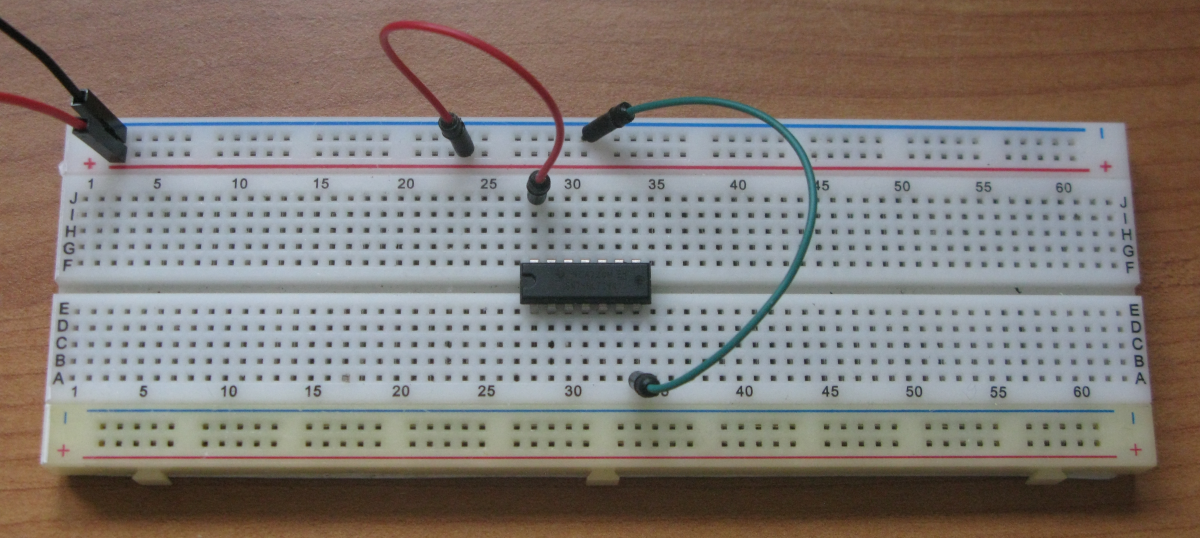
\includegraphics[width=0.95\textwidth]{warsztat_elektroniczny/dip_ic}\\
  Tak umieszczamy układy scalone w płytce stykowej. Dzięki temu każdy z pinów ma połączenie z oddzielną kolumną otworków na płytce.
\end{center}\end{Ramka}\end{figure}

Umieszczając inne elementy w płytce stykowej należy pamiętać, jak połączone są otworki - to znaczy, że jeżeli chcemy
połączyć dwa elementy, to ich odpowiednie ``nóżki'' muszą być umieszczone w tej samej kolumnie. Można też połączyć dwie kolumy otworków
ze sobą za pomocą pasujących kabelków.
\\

Na brzegach płytki najczęściej znajdują się podłużne listwy z takimi samymi otworkami, co reszta płytki, pogrupowanymi w grupy 2x5.
Niektóre płytki posiadają też nadrukowane kreski oraz znaki + i -. Te listwy służą do doprowadzania
zasilania do układu na płytce. Otworki w jednej linii wzdłuż płytki są połączone elektrycznie - tworzą tzw.
\textbf{szynę zasilania}. Z reguły umieszczane są w parach - jedna szyna dla dodatniego napięcia, a druga dla ujemnego (masy).\\

Jeżeli twoja płytka ma nadrukowane oznaczenia wzdłuż tych szyn, to napięcia zasilania (+ oraz -) z przetwornicy należy podłączać zgodnie z~tymi
oznaczeniami. Zmniejsza to ryzyko kosztownej pomyłki.\\

W niektórych płytkach szyny zasilania są rozdzielone w połowie. Należy o tym pamiętać, ponieważ nie ma na to reguły.
Możesz sprawdzić czy Twoja płytka ma rozdzielone szyny za pomocą multimetru (w trybie omomierza lub testu przewodnictwa). Pozwoli to uniknąć
niespodzianek przy prototypowaniu.

\begin{ProTip}{\normalfont{\strong{Uwaga}}}
  Przed wprowadzaniem jakichkolwiek zmian na płytce stykowej odłącz zasilanie. Pozwoli to uniknąć przypadkowych zwarć i uszkodzeń elementów.
\end{ProTip}

\begin{Zadanie}{}{}
  Za pomocą funkcji testu połączeń swojego miernika, sprawdź, czy Twoja płytka stykowa ma rozdzielone szyny zasilania.
  \textit{Wskazówka: Użyj odpowiednich kabelków żeby podłączyć sondy miernika do szyn na płytce - jeden koniec kabelka włóż do płytki a drugim
    dotknij do sondy miernika.}
\end{Zadanie}

\begin{Zadanie}{}{}
  Znajdź w swoim zestawie opornik 1k$\Omega$ (możesz użyć do tego multimetru, ale pamiętaj, że oporniki mają typową tolerancję 5\Verb$%$,
  więc jest mało prawodopodobne, że znajdziesz opornik który ma dokładnie 1000$\Omega$). Jaki prąd popłynie, gdy podłączysz go do napięcia 9V?
  Potwierdź swoje obliczenia za pomocą pomiaru multimetrem.
\end{Zadanie}

\begin{Zadanie}{}{}
  Jaka moc wydzieli się na oporniku z poprzedniego zadania?
\end{Zadanie}
